\documentclass[10pt, a4paper]{article}
\usepackage[polish]{babel}
\usepackage[utf8]{inputenc}
\usepackage{graphicx} 
\usepackage{amsmath}
\usepackage{amsthm}
\usepackage{amssymb}
\usepackage{mathtools}
\usepackage[utf8]{inputenc}
\usepackage[left=2cm, top=-5cm, right=2cm, bottom=2cm, includeheadfoot, headheight=130pt, a4paper]{geometry}
\usepackage[polish]{babel}
\usepackage[utf8]{inputenc}
\usepackage{polski}
\usepackage[T1]{fontenc}
\usepackage{longtable}
\usepackage{caption}
\usepackage{subcaption}
\usepackage{booktabs}
\usepackage{array}
\usepackage{etoolbox}
\usepackage{xcolor}
\usepackage{listings}
\usepackage{multicol}
\usepackage{float}
\usepackage{hyperref}

\BeforeBeginEnvironment{verbatim}{\small}
\lstset{language=c++,
                basicstyle=\ttfamily\footnotesize,
                keywordstyle=\color{blue}\ttfamily\footnotesize,
                stringstyle=\color{red}\ttfamily\footnotesize,
                commentstyle=\color{green}\ttfamily\footnotesize,
                morecomment=[l][\color{magenta}]{\#},
                extendedchars=true,
                literate={ą}{{\k{a}}}1 {ć}{{\'c}}1 {ę}{{\k{e}}}1 {ł}{{\l{}}}1 {ń}{{\'n}}1 {ó}{{\'o}}1 {ś}{{\'s}}1 {ź}{{\'z}}1 {ż}{{\.z}}1
                         {Ą}{{\k{A}}}1 {Ć}{{\'C}}1 {Ę}{{\k{E}}}1 {Ł}{{\L{}}}1 {Ń}{{\'N}}1 {Ó}{{\'O}}1 {Ś}{{\'S}}1 {Ź}{{\'Z}}1 {Ż}{{\.Z}}1
}

\title{Wybrane Zagadnienia Algebry\\Sprawozdanie 3}
\author{Rafał Włodarczyk 279762}
\date{Czerwiec 2026}

\begin{document}

\maketitle

\section{(a)}

\section{(b)}

\section{(c) Układy Równań}

\subsection{Układ Pierwszy}

\begin{figure}[H]
\begin{minipage}[b]{0.74\textwidth}  
Baza Grobnera dla następującego układu równań:
\begin{align*}
\begin{cases}
x^2+y^2=z^2 \\
(c+1)z = 0
\end{cases}
\xRightarrow[\text{z > x > y}]{\text{GrobnerBasis}}
\begin{cases}
x^2 + y^2 \\
z
\end{cases}
\\
\implies
\mathcal{I}_f = x^2 + y^2
\end{align*}
Drugie równanie $10z=0$ wymusza $z=0$, więc jedynym rozwiązaniem jest punkt.

\end{minipage}
\begin{minipage}{0.24\textwidth}  
    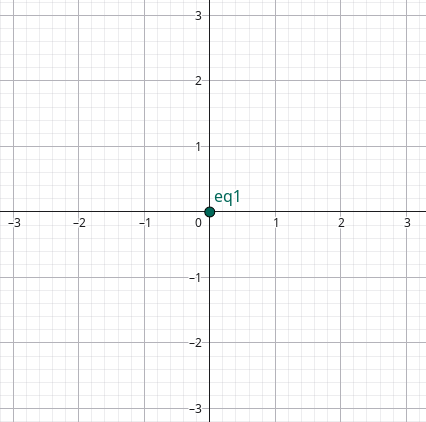
\includegraphics[width=0.99\linewidth]{ex-c-1.png}
    \captionof{figure}{$\mathcal{V}(x^2+y^2)$}
\end{minipage}
\end{figure}

\subsection{Układ Drugi}

\begin{figure}[H]
\begin{minipage}[b]{0.74\textwidth}  
Baza Grobnera dla następującego układu równań:
\begin{align*}
\begin{cases}
x^2 + y^2 = z^2 \\
z + 8 = 0
\end{cases}
\xRightarrow[\text{z > x > y}]{\text{GrobnerBasis}}
\begin{cases}
x^2 + y^2 - 64 \\
z + 8
\end{cases}
\\
\implies
\mathcal{I}_f = x^2 + y^2 - 64
\end{align*}
Drugie równanie $z=-8$ sprawia, że zbiór rozwiązań jest równaniem okręgu.

\end{minipage}
\begin{minipage}{0.24\textwidth}  
    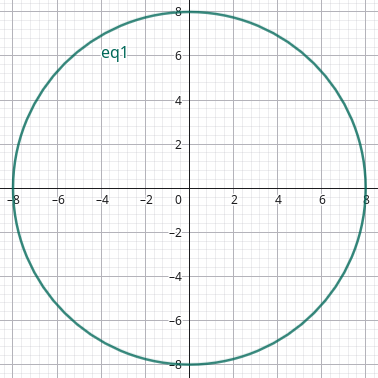
\includegraphics[width=0.99\linewidth]{ex-c-2.png}
    \captionof{figure}{$\mathcal{V}(x^2+y^2 - 64)$}
\end{minipage}
\end{figure}

\subsection{Układ Trzeci}

\begin{figure}[H]
\begin{minipage}[b]{0.74\textwidth}  
Baza Grobnera dla następującego układu równań:
\begin{align*}
\begin{cases}
x^2 + y^2 = z^2 \\
x + z + 5 = 0
\end{cases}
\xRightarrow[\text{z > x > y}]{\text{GrobnerBasis}}
\begin{cases}
x + z + 5 \\
y^2 + 10z + 25
\end{cases}
\\
\implies
\mathcal{I}_f = y^2 + 10 (-x -5) + 25 = y^2 - 10x - 25
\end{align*}
\end{minipage}
\begin{minipage}{0.24\textwidth}  
    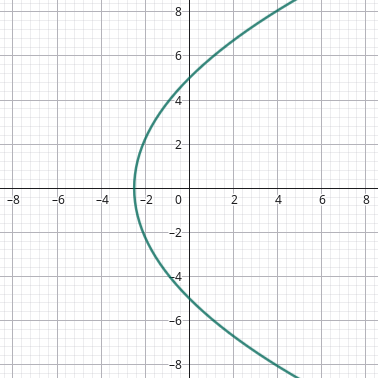
\includegraphics[width=0.99\linewidth]{ex-c-3.png}
    \captionof{figure}{$\mathcal{V}(y^2 - 10x - 25)$}
\end{minipage}
\end{figure}

\subsection{Układ Czwarty}

\begin{figure}[H]
\begin{minipage}[b]{0.74\textwidth}  
Baza Grobnera dla następującego układu równań:
\begin{align*}
\begin{cases}
x^2 + y^2 = z^2 \\
x + y + z + 3 = 0
\end{cases}
\xRightarrow[\text{z > x > y}]{\text{GrobnerBasis}}
\begin{cases}
x + y + z + 3 \\
y^2 + yz + 3y + 3z + 4.5
\end{cases}
\\
\implies
\mathcal{I}_f = y^2 + z (y + 3) + 3y + 4.5 =\\
= y^2 + (-3-y-x) (y + 3) + 3y + 4.5 =\\
= -4.5 -3x -3y - xy
\end{align*}
\end{minipage}
\begin{minipage}{0.24\textwidth}  
    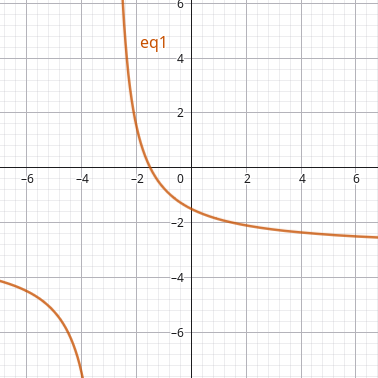
\includegraphics[width=0.99\linewidth]{ex-c-4.png}
    \captionof{figure}{$\mathcal{V}(-4.5 -3x -3y - xy)$}
\end{minipage}
\end{figure}

\subsection{Układ Piąty}

\begin{figure}[H]
\begin{minipage}[b]{0.74\textwidth}  
Baza Grobnera dla następującego układu równań:
\begin{align*}
\begin{cases}
x^2 + y^2 = z^2 \\
y + 2z + 2
\end{cases}
\xRightarrow[\text{z > x > y}]{\text{GrobnerBasis}}
\begin{cases}
x^2 + 3z^2 + 8z + 4
y + 2z + 2
\end{cases}
\\
\implies
\mathcal{I}_f = x^2 + 3(-2-y)^2 + 8(-2-y) + 4 =\\
= x^2 + 3 y^2 + 4 y
\end{align*}
\end{minipage}
\begin{minipage}{0.24\textwidth}  
    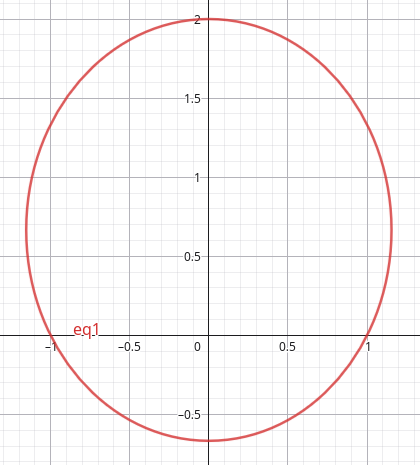
\includegraphics[width=0.99\linewidth]{ex-c-5.png}
    \captionof{figure}{$\mathcal{V}(x^2 + 3 y^2 + 4 y)$}
\end{minipage}
\end{figure}

\section{(d) Baza oraz Eliminacja zmiennej}

Dla zadanego układu wyznaczam Bazę Grobnera przy użyciu mojej implementacji algorytmu Buchbergera. 
\begin{align*}
    \begin{cases}
        (x^2+y^2-ax)^2 = z^2(x^2+y^2)\\
        x+2y+3z = 0
    \end{cases}
\end{align*}
Koduję wejście - wielomiany wielu zmiennych:
\begin{figure}[h]
\begin{minipage}[t]{0.49\textwidth}   
\begin{lstlisting}{c++}
const poly_t D1 = {
    {{2, 0, 0}, a * a},
    {{3, 0, 0}, -2 * a},
    {{1, 2, 0}, -2 * a},
    {{4, 0, 0}, 1},
    {{2, 2, 0}, 2},
    {{0, 4, 0}, 1},
    {{2, 0, 2}, -1},
    {{0, 2, 2}, -1}
};
\end{lstlisting}
\end{minipage}
\begin{minipage}[t]{0.49\textwidth}   
\begin{lstlisting}{c++}
const poly_t D2 = {
    {{1, 0, 0}, 1},
    {{0, 1, 0}, 2},
    {{0, 0, 1}, 3}
};
\end{lstlisting}
\end{minipage}
\end{figure}\\
Wynik działania programu:
\begin{verbatim}
Grobner basis von
(x^4) - 4(x^3) + 2(x^2)(y^2) 
- (x^2)(z^2) + 4(x^2) - 4(x)(y^2) 
+ (y^4) - (y^2)(z^2) 
und
(x) + 2(y) + 3(z)
Computed Groebner basis:
1. (x) + 2(y) + 3(z)
2. (y^4) + 4.80(y^3)(z) + 1.60(y^3) + 9.160(y^2)(z^2) 
   + 6.240(y^2)(z) + 0.640(y^2) + 8.160(y)(z^3) 
   + 8.640(y)(z^2) + 1.920(y)(z) + 2.880(z^4) + 4.320(z^3) + 1.440(z^2)
\end{verbatim}
Wybieramy drugie wyrażenie, nieposiadające zmiennej $x$. W celu wykonania wykresu tego równania $w(y,z)=0$
wprowadzamy podstawienie $x \gets y, y \gets z$ i rysujemy w układzie kartezjańskim $(x,y)$.
\begin{align*}
    0.64x^{2}+1.6x^{3}+1x^{4}+1.92xy+6.24x^{2}y+4.8x^{3}y+1.44y^{2}+8.64xy^{2}+9.16x^{2}y^{2}+4.32y^{3}+8.16xy^{3}+2.88y^{4}=0
\end{align*}
\noindent
W tym podpunkcie należy również porównać wynik z podstawieniem $z=a$ do pierwszego z równań, zachodzi:
\begin{align*}
    (*) \quad (x^2+y^2-ax)^2 = a^2(x^2+y^2) 
\end{align*}
Kolorem czerwonym oznaczona jest krzywa policzona za pomocą bazy Grobnera.
Kolorem niebieskim oznaczone jest równianie $(*)$, dla $a=2$.
\begin{figure}[H]
    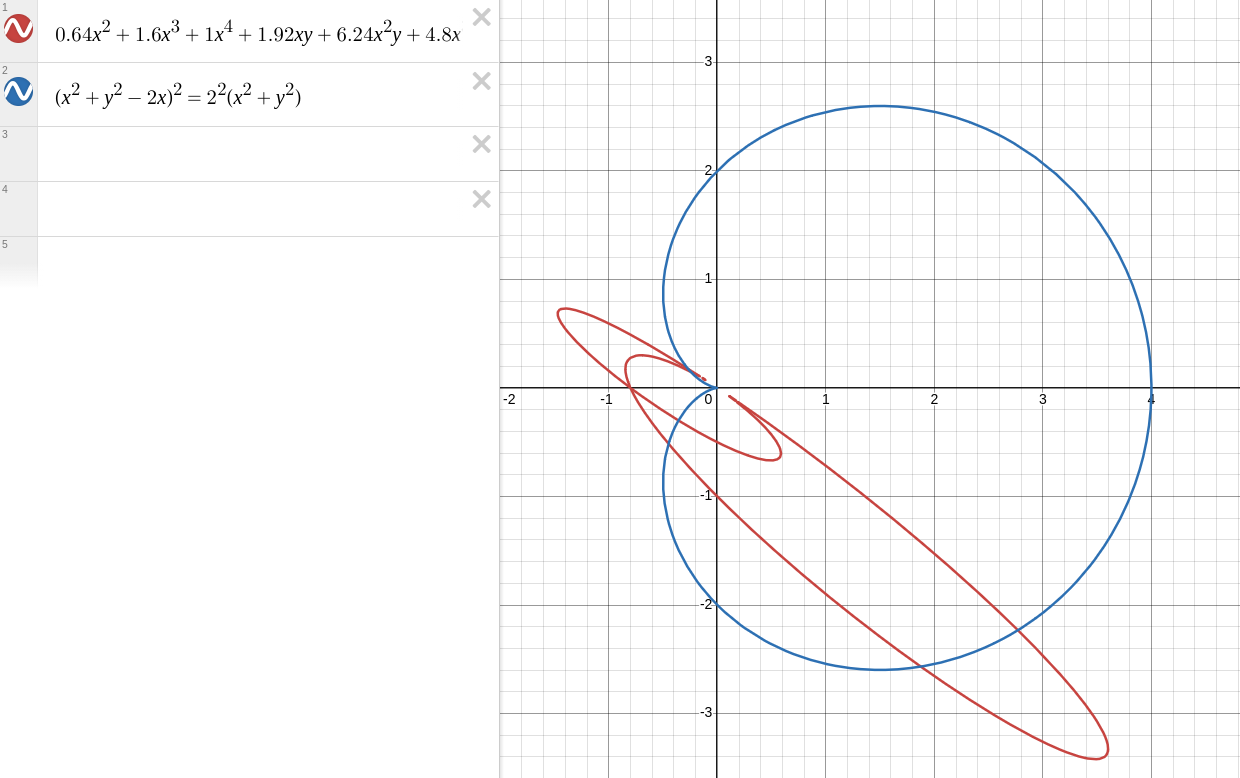
\includegraphics[width=0.99\linewidth]{ex-d.png}
\end{figure}

\section{(e) Baza Grobnera oraz Trysektrysa}

Dla zadanej funkcji w układzie biegunowym wprowadzamy podstawienie
 $\cos (\theta) = \frac{x}{r}$, tak jak na poprzedniej liście w celu przejścia do układu kartezjańskiego.
\begin{align*}
    r = b \left(4 \cos (\theta) + \frac{1}{\cos (\theta)}\right)
    &= b \left(4 \frac{x}{r} + \frac{r}{x}\right)\\
    b \left(\frac{4x^2 + r^2}{rx}\right) - r &= 0 \\
    b (4x^2 + r^2) - r^2 x &= 0 \\
    b r^2 + 4bx^2 - r^2 x &= 0
\end{align*}
Mamy następujący układ równań:
\begin{align*}
    \begin{cases}
        x^2 + y^2 - r^2 = 0 \\
        b r^2 + 4b x^2 - r^2 x = 0
    \end{cases}
\end{align*}
Wyciągnijmy z pomocą Bazy Grobnera wyrażenia zawierające jedynie $x,y$. Wynik działania programu:

\begin{verbatim}
Grobner basis von -(r^2) + (y^2) + (x^2) und -(r^2)(x) + 7(r^2) + 28(x^2)
Computed Groebner basis:
1. (r^2) - (y^2) - (x^2)
2. (y^2)(x) - 7(y^2) + (x^3) - 35(x^2)
\end{verbatim}
Zauważmy, że drugi element bazy składa się tylko z $x,y$. Jest on zatem naszym rozwiązaniem:
\begin{align*}
    f(x,y) = y^2\cdot x -7y^2 + x^3 - 35x^2 = 0
\end{align*}

\subsection{Wykresy Trysektrysy}

Po lewej stronie narysowałem krzywą w Geogebrze za pomocą wyjściowego równania $r(\theta)$ w układzie biegunowym. Po prawej stronie
narysowałem te samą krzywą za pomocą równania dwóch zmiennych $f(x,y)=0$

\begin{figure}[H]
    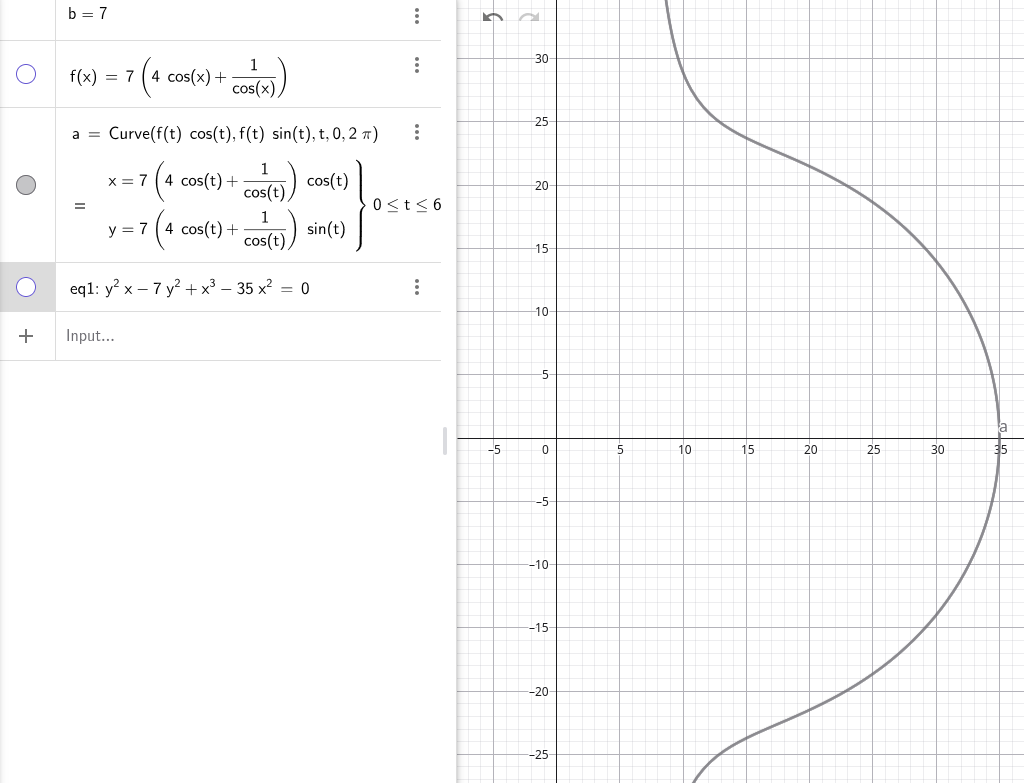
\includegraphics[width=0.49\linewidth]{ex-e-rcurve.png}
    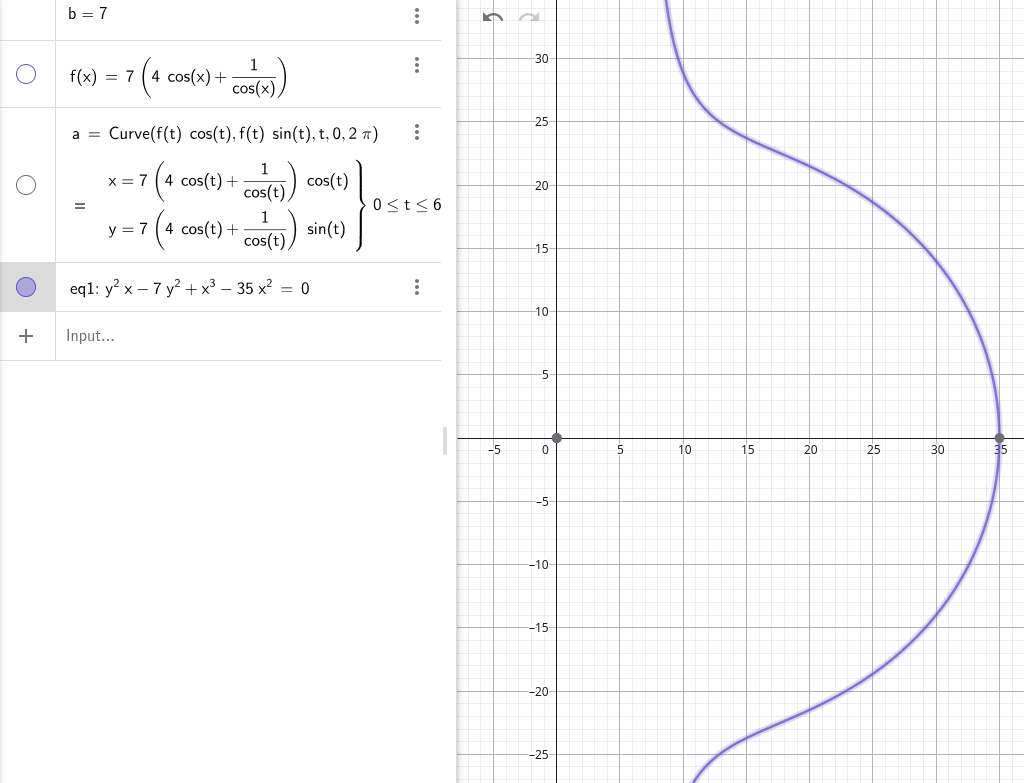
\includegraphics[width=0.49\linewidth]{ex-e-poly.png}
\end{figure}


\end{document}